
\chapter[Introduction]{Introducción: importancia de \LaTeX{} para las humanidades}


\section{Una carencia importante}

Este libro es el resultado de año y medio de trabajo y del uso diario de \LaTeX para la redacción de nuestro proyecto de fin de carrera. A nuestro juicio, viene a colmar un vacío. Efectivamente, aunque las obras sobre \LaTeX son numerosas, son pocas las que se destinan específicamente a las humanidades. 

Aunque la palabra \LaTeX ya la hayan oído mencionar oídos humanistas, evoca ---salvo raras excepciones---  en el mejor de los casos, una herramienta para las ciencias llamadas duras, y en el peor, la savia de un árbol o un plástico con múltiples aplicaciones. 

Algunas razones podrían explicar este semivacío:
\begin{itemize}
\item una tendancia de los estudiosos de humanidades a conocer mal o a ignorar las herramientas informáticas;
\item \LaTeX parece \emph{de entrada} poco amigable;
\item durante mucho tiempo \LaTeX no ha tenido herramientas para festionar de forma adecuada y sencilla una bibliografía de acuerdo con las normas propias de las humanidades: notas a pie de página, distinción entre fuentes primarias y secundarias, etc.;
\item hubo un tiempo en que la gestión de los caracteres no latinos no era de las cosas más sencillas en \LaTeX ;
\item Los editores de humanidades no suelen aceptar textos formateados en \LaTeX porque los autores no suelen componerlos en \LaTeX porque los editores no suelen aceptarlos en \LaTeX\ldots
\end{itemize}

Como los estudiosos de humanidades son especialistas en el escrito, durante un tiempo los únicos programas de tratamiento de texto, como  LibreOffice.org o Microsoft Word, fueron los únicos que se emplearon para redactar trabajos académicos.

Y eso es una paradoja: en efecto, como acabamos de ver, estos procesadores de texto tienen defectos importantes que deberían estimular a los autores a cambiarlos. 

\section{¿Por qué \LaTeX{} ?}

\subsection{Desventajas de los procesadores de texto}

Cuando escribes en tu procesador de texto, como, por ejemplo, Microsoft Word o LibreOffice.org, éste ejecuta dos acciones a la vez:
\begin{itemize}
\item por una parte, almacena en un fichero la estructura lógica de tu trabajo: encabezados, párrafos, notas a pie de página, etc.;
\item por otra parte, te muestra en la pantalla la representación \enquote{física} de tu texto (justificación, negritas, cursivas, etc.), tal como lo dispondría un lector.
\end{itemize}

Por este motivo este tipo de programas se llaman WYSIWYG, que en inglés es el acrónimo de \textenglish{\emph{What You See Is What You Get}}\footnote{\enquote{Lo que ves es lo que obtienes}.}. 

Esta combinación de dos funciones distintas en los procesadores de texto implica tres consecuencias:
\begin{itemize}
\item La necesidad de mostrar en tiempo real la representación física del texto mientras se mantiene una alta velocidad del programa tiene como consecuencia una disminución de la calidad tipográfica. Por ejemplo:
	\begin{itemize}
	\item Para tener un texto justificado a izquierda y derecha, los procesadores de texto varían el tamaño de los espacios entre palabras. Las variaciones son, en ocasiones, considerables, cosa que puede disminuir la comodidad de la lectura. Para evitar este tipo de problemas, los libros clásicos cortan las palabras al final de la línea, lo que se llama partición\footnote{La partición silábica no se hace en cualquier lugar: debe respetar las reglas propias de cada lengua.}.
\item Los espacios en blanco situados delante de algunos signos de puntuación, como, por ejemplo, los signos de exclamación, son del mismo tamaño que los espacios que separan las palabras, mientras que las normas tipográficas clásicas prevén espacios más pequeños.\footnote{Esto es así para la tipografía francesa, pero no para la española (Nota del Traductor).}
	\end{itemize}
\item El hecho de que un mismo programa se ocupe \emph{a la vez} de la visualización y de la estructura del texto, tiende a confundir ambos\footcite[El autor de estas líneas es menos reticente a los procesadores de texto que otros LaTeXeros : \cf][]{stupide}  :
	\begin{itemize}
\item Este tipo de prácticas anima a concentrarse en la forma más que en el contenido y la estructura\footcite[No obstante, en teoría, la formación universitaria en humanidades anima a pensar \emph{primero, estructura y sentido}. Véase una discusión en el blog del autor:][]{structurevsforme}. 
\item Los autores no usan siempre la posibilidad de separar forma y contenido por medio de los estilos. En ese caso, cuando se quiere cambiar la forma de un elemento lógico, como el título de un capítulo, hay que cambiar todos los lugares donde se utiliza ese elemento lógico\footnote{Por ejemplo, alguien que no haya usado los estilos para diseñar sus títulos de capítulo, tendrá que seleccionar \emph{todos los títulos de capítulos}, después ir a los menús de formato, etc.}.
	\end{itemize}
\item Los pesados cálculos informáticos necesarios para el formato en tiempo real hacen a los procesadores de textos muy lentos en comparación con otros programas. Esta lentitud se convierte a menudo en una fuente de enfado y de pérdida de concentración. Además, estos programas exigen muy a menudo material reciente.
\end{itemize}

Por otra parte, aunque los procesadores de textos recientes disponen de herramientas para gestionar la bibliografía, éstas suelen carecer de flexibilidad; por eso se utilizan pocas veces\footnote{Siempre se puede recurrir a herramientas externas, como EndNote o Zotero.}. Por tanto, son muchos los autores que escriben su bibliografía \enquote{a mano} tecleando directamente: Nombre del autor, \emph{Título}, etc. En caso de error, hay que corregir todos los lugares en que se cita la obra.

\subsection{Ventajas de \LaTeX{}}

\LaTeX{} permite resolver todos los problemas de los procesadores de texto. Efectivamente, separa dos etapas:
\begin{itemize}
\item La etapa de redacción, que ocurre en un editor de texto. El autor introduce su texto e indica, mediante algunos comando, su estructura (encabezados, párrafos, notas a pie de página).
\item La etapa de cálculo del resultado final sólo se hace después: el autor pasa su fichero por un compilador\footnote{Que se puede describir a grandes rasgos como un conjunto de órdenes informáticas destinadas a producir un objeto informático a partir de un lenguaje más fácil de leer para los humanos.}, en ocasiones también llamado compositor\footnote{En realidad, el término \forme{compositor} es más correcto, desde el punto de vista del vocabulario informático, que el término \forme{compilador}. No obstante, éste último se emplea con más frecuencia en la lengua corriente.}. Este último programa lee el conjunto de los comandos del archivo para producir un nuevo archivo con formato PDF\footnote{Históricamente \LaTeX{} producía otro formato de fichero: DVI. Pero para nuestro objetivo, esto carece de importancia: en este libro sólo utilizaremos la producción de PDF.}.
\end{itemize}

Esta separación permite:
\begin{itemize}
\item  Una calidad tipográfica superior:  como el compilador no se ve obligado a una presentación en tiempo real, puede hacer cálculos más pesados: así, por ejemplo, \LaTeX{} produce cortes de palabras tipográficos y no espacios en blanco de geometría variable, y equilibra mejor la composición del texto.
\item Una mejor separación del sentido y de la forma, ya que el autor da solamente indicaciones de sentido.
\end{itemize}

Además, \LaTeX{} tiene un sistema de gestión de la bibliografía extremadamente potente que permite al autor separar el contenido de su bibliografía\footnote{Títulos, autores, etc.} de su presentación\footnote{¿Hay que poner \emph{op. cit.}?; y si hay que hacerlo, ¿dónde?¿Hay que poner sólo las iniciales de los nombres o los nombres completos?, etc.}.

Esta separación entre el contenido de la bibliografía y la presentación no sólo resulta útil a los autores, sino también a los editores. En efecto, si el autor estructura correctamente su base de datos bibliográfica\renvoi{bddbiblio}, el editor puede adaptar la presentación de la bibliografía a sus propias reglas: le basta con crear archivos de estilos bibliográficos siguiendo una sintaxis sencilla.

La gestión de una bibliografía es, a la vez, uno de los trabajos más importantes en humanidades, y uno de los más difíciles, con muchas fuentes posibles de errores. Esta sencilla razón basta, en opinión del autor, para preferir \LaTeX{} a un programa de tratamiento de texto\footnote{El autor y su hermana se han decidido a utilizar \LaTeX{} en el ámbito de sus trabajos universitarios, y el elemento detonante de la elección ha sido la facilidad y flexibilidad de la gestión bibliográfica.}.

Otra ventaja de  \LaTeX{} es la producción directa de un documento en formato PDF. Cuando se reciben documentos en formato digital, es muy frecuente que, al abrir el fichero, se pierda el formado, que la impresión sea de mala calidad o incluso que resulte totalmente imposible abrir el fichero.

El \emph{\textenglish{Portable Document Format}} permite evitar estos inconvenientes. Se trata de un formato abierto, es decir, que su creador,  la sociedad Adobe, ha publicado todas las especificaciones necesarias para la creación de programas que puedan leer este formato. Por tanto, hay muchos lectores de PDF que se pueden emplear en numerosos sistemas operativos\footnote{Para una introducción a los lectores libres y gratuitos disponibles para tu sistema operativo, si no tienes uno ya, dirígete a la página \url{http://pdfreaders.org/index.es.html} (en español).}.

El formato PDF está diseñado para que se pueda leer de forma universal. En efecto, incrusta en un mismo archivo no sólo el texto y las imágenes que pueda haber, sino también las indicaciones del diseño de página y de las fuentes. También garantiza totalmente que quien vea tu documento o lo lea impreso verá exactamente lo que tenías en mente a la hora de componerlo, cosa que constituye una ventaja innegable respecto a los formatos de archivos tales como los de Microsoft Word, por ejemplo. Además, tienes la seguridad de que el PDF que conserves es eterno. En la medida en que cualquiera es libre de desarrollar un programa que permita la lectura de los PDF y que las especificaciones son de acceso libre, tienes la garantía de que el destino de tus publicaciones no dependerá de la buena voluntad de un vendedor de programas en el curso de los años, lo que hace de PDF un formato ideal para archivar publicaciones.

Lamentablemente, la moneda tiene su cruz: aunque es un formato de archivo legible universalmente, el PDF es difícil de modificar cómodamente: no está pensado para ese uso. Por tanto, si quieres trabajar en colaboración sobre un libro utilizando \LaTeX, tendrás que trabajar de forma distinta\renvoi{principesvn}.

\subsection{¿Qué es un editor de texto?}

Hemos hablado en los párrafos anteriores de dos tipos de programas que no hay que confundir:
\begin{enumerate}
	\item Los procesadores de texto.
	\item Los editores de texto.
\end{enumerate}

Hemos visto lo que eran los primeros: programas que se encargan de incluir en un archivo la estructura lógica de un texto y de mostrar su apariencia física. Los segundos son sencillamente programas que permiten a una persona escribir en un archivo texto y ponerle él mismo sus comandos de estructuración. No obstante, los buenos editores de texto hacen más que eso, ayudan a escribir con diversas herramientas:
\begin{itemize}
\item con frecuencia colorean en la pantalla los comandos para permitir que se vean mejor: es lo que se llama resaltado de sintaxis;\label{colorationsyntax}
\item ofrecen ayuda para teclear los comandos más frecuentes:  atajos de teclado, botones, etc.;
\item a veces, ofrecen una visión del plan del trabajo.
\end{itemize}

Algunos de esos editores de texto son generales y se adaptan a muchos lenguajes de programación\footnote{Por ejemplo,  \LaTeX{} y HTML, el último de los cuales se emplea para los sitios de internet.}. Otros están especializados en un lenguaje en particular: en ese caso, ofrecen herramientas adicionales específicas para el lenguaje en que están especializados. 

Así, los editores especializados en  \LaTeX{} ofrecen botones específicos para ejecutar el compilador  \LaTeX{}.

Par empezar en \LaTeX{} tendrás, por tanto, que abandonar tu viejo procesador de texto y elegir un editor de texto especializado en \LaTeX{}: te damos una lista de algunos en el anexo\renvoi{editeurs}.

\section[TeX, LaTeX, XeTeX, XeLaTeX: puntos comunes y diferencias]{\TeX{}, \LaTeX{}, \XeTeX{} et \XeLaTeX{}: puntos comunes y diferencias}\label{TeXLaTeX}

En este capítulo hemos hablado de \LaTeX{}. Sin embargo, el título de este libro habla de \XeLaTeX{}. ¿Cuál es la diverencia? Veamos una breve explicación histórica muy simplificada\footnote{El lector que tenga curiosidad puede encontrar con facilidad documentación más detallada sobre este tema, sobre todo, en Internet.}.

\begin{enumerate}
\item En 1977 Donal Knuth inventó  \TeX{} que era un sencillo maquetador de texto, capaz de transformar un texto estructurado con comandos en un texto con formato. Con \TeX{} también se podían crear comandos propios.
\item El uso de \TeX{} era relativamente complicado. Leslie Lamport creó un conjunto de comandos \TeX{} para simplificar su uso . Este conjunto de comandos permitió formar el lenguaje \LaTeX{} y su respectivo compilador.
\item A continuación, se creó un compilador derivado de \TeX{}: \XeTeX{}. Permite dos cosas:
\begin{itemize}
	\item una gestión del conjunto de las escrituras mundiales por medio del conjunto de caractéres Unicode\renvoi{utf8};
	\item una gestión de las nuevas fuentes de formato OpenType\footnote{Este tipo de fuente permite, por ejemplo, una gestión potente de las ligaduras entre las letras.}, que aparecieron a principios de los 2000.

\end{itemize} 
\item Para poder usar los comandos de \LaTeX{} con \XeTeX{} se ideó \XeLaTeX{}.
\end{enumerate}

Se pueden resumir las relaciones entre \TeX{}, \LaTeX{}, \XeTeX{} y \XeLaTeX{} con el esquema~\ref{sch:tex} (p.~\pageref{sch:tex}).

\begin{figure}[ht]
\centering
% Schéma des parentes entres TeX LaTeX XeTeX etc.
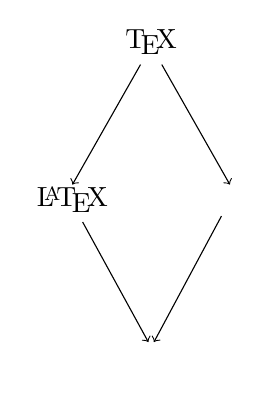
\begin{tikzpicture}
	
	% Les textes
	\node[text height=1ex,anchor=mid] (T) at (0,0) 		 	{\TeX} ;
	\node[text height=1ex,anchor=mid]  (X) at (1, -2)	 	 	{\XeTeX};
	\node[text height=1ex,anchor=mid]  (L) at (-1, -2) 		{\LaTeX};
	\node[text height=1ex,anchor=mid]  (XL) at (0,-4)			{\XeLaTeX};
	
	% Les traits
	\draw[->] (T) -- (X.north);
	\draw[->] (T) -- (L.north);
	\draw[->] (L) -- (XL.100);
	\draw[->] (X) -- (XL.80);
\end{tikzpicture}

\caption{Relaciones entre \TeX{}, \LaTeX{}, \XeTeX{} y \XeLaTeX{}}\label{sch:tex}
\end{figure} 

En este libro trabajaremos sobre \XeLaTeX{}. Pero, como la mayoría de nuestros planteamientos se pueden aplicar indistintamente a  \LaTeX{} y a \XeLaTeX{}, utilizaremos el término \forme{\LaTeX{}}, salvo cuando señalemos una característica específica de \XeLaTeX{}.
%%%%%%%%%%%%%%%
\begin{plusloins}
Aunque el tema es objeot de debate, parece que hay que pronunciar la \forme{X} de \TeX{} como una \forme{χ} griega, pues el nombre \TeX{} procedería de la palabra griega \forme{\textgreek{τέχνη}} : \forme{arte, ciencia}. Ainsi prononcerait-on \forme{latek}.
\end{plusloins}


\section{Público al que se dirige esta obra}

Esta obra se dirige a tres públicos diferentes.

Ante todo, a los estudiantes e investigadores de humanidades que no se arredran ante la idea de aprender una nueva herramienta informática que, aunque les parezca que pierden tiempo con ella al principio,les hará ganar un tiempo precioso con el uso.

A continuación, a los editores de revistas y de libros de humanidades, para animarlos a que tengan en cuenta \LaTeX cuando elijan sus formatos de archivo, y para mostrarles la ventaja de este formato respecto a los demás. Esperamos demostrar que \LaTeX permite resolver muchos problemas de edición, en especial en lo que atañe a las normas bibliográficas, ya que distingue con nitidez el sentido y la forma.

Por último, a los usuarios de \LaTeX que proceden de las ciencias llamadas \enquote{duras}, para mostrarles las características editoriales de las humanidades y la necesidad de extensiones ---llamadas \forme{package} en \LaTeX{}--- adaptadas.


\section{Cómo leer este libro}

Esta obra no es un manual sobre \LaTeX{}. Se considera más bien una introducción y no tiene más objetivo que presentar los fundamentos de \LaTeX{}. Una vez adquiridos, el lector-redactor debería ser capaz de comprender la lógica de \LaTeX{} y, luego, poder encontrar con facilidad las informaciones útiles para su proyecto.

Es evidente que estos fundamentos no son los mismos que los que presentan otros libros de introducción a \LaTeX{}, orientados, por lo general, a las ciencias llamadas duras. Por eso no encontrarás en el la forma de incluir una ecuación. Sin embargo, describimos en él distintos elementos que, con fracuencia, se tocan muy de pasada en las demás introducciones: las distintas formas de hacer una cita, de indicar un cambio de lengua, la manera de escribir en uno o más alfabetos no latinos,etc.

La primera parte se dedicará a presentar los principios de funcionamiento de \LaTeX. El capítulo primero, en forma de tutorial, tiene como objetivo presentar los conceptos esenciales. El resto de capítulos, más formales, describen las herrmientas fundamentales y exigen haber comprendido los conceptos. Sin embargo, el orden de lectura depende sustancialmente de las necesidades editoriales del lector. 

Éste podría, sin duda, comenzar por los primeros capítulos de la segunda parte, que presenta las herramientas de gestión bibliográfica en \LaTeX{}, comenzando por la creación de la base de datos bibliográfica.

La tercera parte trata de introducir el conjunto de las herramientas necesarias para facilitar la navegación en el trabajo final: contenidos, referencias cruzadas, índices.

La cuarta introduce herramientas de \LaTeX{} que el autor ha considerado que podrían ser especialmente útiles en humanidades.

Como la distinción entre forma y sentido está en el núcleo de la lógica de  \LaTeX{}, hemos considerado importante no tocar, de manera resumida, las cuestiones del formateado más que en la última parte\footnote{Con excepción de un capítulo concreto de la primera parte, pero que toca ante todo las cuestiones de dar sentido.}.

El lector nos perdonará por no haber incluido una conclusión, pero la naturaleza de este libro no se presta a ello.No obstante, encontrará algunos anexos que incorporan,además de los índices indispensables y bibliografías, varias informaciones útiles:  cómo instalar y actualizar \LaTeX{}, cómo encontrar ayuda, una presentación de algunos programas relacionados con \LaTeX{}, un glosario, una presentación de herramientas útiles para que trabajen varias personas en un mismo proyecto.

Cada capítulo de este libro comienza con una breve introducción en la que se indica su objetivo así como los conocimientos previos necesarios para comprenderlo. A lo largo del texto aparecen dos tipos de llamadas: llamadas de \enquote{atención}, marcadas con relámpagos y cuyo significado no merece la pena explicar, y llamadas \enquote{para ir más lejos}, marcadas con huellas y que pretenden satisfacer la curiosidad el lector y el placer de la digresión del autor. Las referencias a otros apartados del libro se indican con la forma (☞\,página, \textbf{capítulo.apartado.subapartado}).

Como las citas que encabezan cada parte no tienen pretensiones cientídicas, los eruditos dispensarán la ligera imprecisión que atañe a su procedencia, ya que no se han determinado con exactitud sus orígenes.

Pedimos excusas, por último, por no especificar los números de página cuando hacemos referencia al manual de un paquete de \LaTeX{}: dada la asiduidad con la que algunos de ellos se actualizan, esta información casi no tendría sentido.
